In this section we evaluate the recorded data.
\subsection{Recorded Energy Spectra}
We recorded the energy spectra of the LYSO-detector itself and that of $^{22}$Na. The spectra recorded with the left detector can be seen in figure \ref{fig:energy_spectra}.

\newpage

\begin{figure}[h]
  \centering
  \begin{subfigure}[h]{0.49\textwidth}
    \centering
    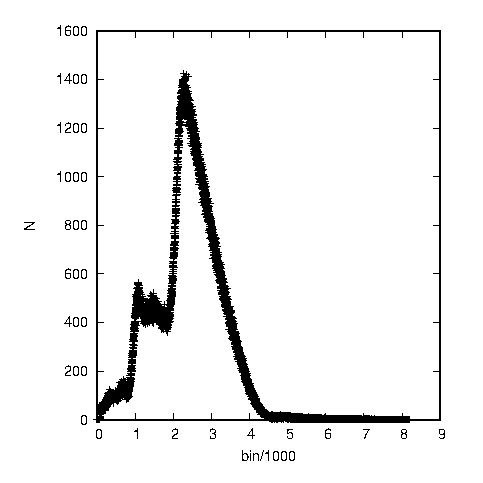
\includegraphics[width=\textwidth]{evaluation_kilian/energy_spectra/links_LYSO.eps}
    \caption{Spectrum of LYSO.}
  \end{subfigure}%
  \begin{subfigure}[h]{0.49\textwidth}
    \centering
    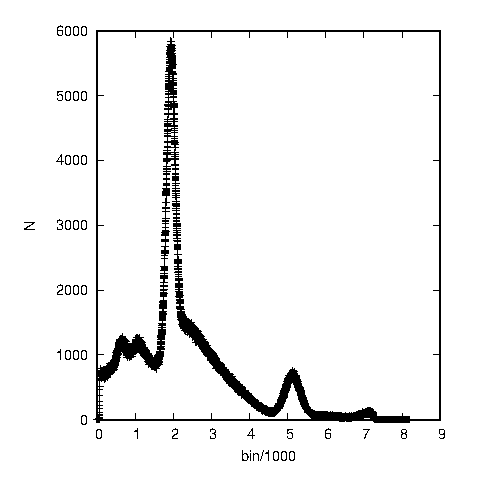
\includegraphics[width=\textwidth]{evaluation_kilian/energy_spectra/links_Na.eps}
    \caption{Spectrum of $^{22}$Na.}
  \end{subfigure}
  \caption{Energy spectra recorded with the left detector.}
  \label{fig:energy_spectra}
\end{figure}

In the LYSO spectrum the main contribution comes from the $6^+ \rightarrow 0^+$ cascade in $^{176}$Hf (see figure \ref{fig:scheme}). In the $^{22}$Na-spectrum there are two peaks we are interested. Namely the \SI{511}{\kilo\electronvolt} line\footnote{From the elcetron-positron annihilation.} around bin 2000 and the \SI{1275}{\kilo\electronvolt} line around bin 5000 from the $2^+ \rightarrow 0^+$ transition. These two peaks are our start- and stop-signal for the lifetime measurement.

\subsection{Time Calibration}
The prompt curve consists of 12 peaks. We fit 12 exponential functions and a background
\begin{align*}
  N(t)=\sum_{i=1}^{12}\frac{A_i}{\sqrt{2\pi\sigma_i^2}}\exp \left( -\frac{(t-\mu_i)^2}{2\sigma_i^2}\right)+C
\end{align*}
to the data, where $t$ is the time in bins of the MCA. For the fitting we use error weighted fitting with gnuplot. The error of $N$ is given by\footnote{We ignore empty bins.} $\sqrt{N}$. The resulting spectrum can be seen in figure \ref{fig:prompt} while the fit-parameters are in table \ref{tab:prompt} in the appendix. Looking at the different widths $\sigma_i$ one can not find an evident bin-dependence of the resolution. We note that the last value $\sigma_{12}$ should be ignored because the peak is cut by the TAC.

\begin{figure}[h]
\centering
\begin{subfigure}[h]{0.49\textwidth}
  \centering
  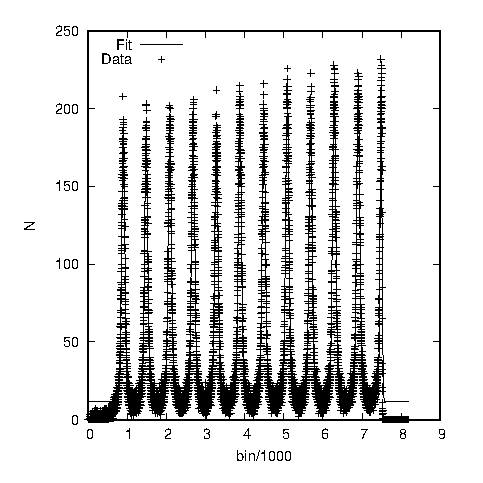
\includegraphics[width=1\linewidth]{evaluation_kilian/prompt/prompt.eps}
  \caption{Prompt curve with fit. For better visibility the error bars are not plotted.}
  \label{fig:prompt}
\end{subfigure}%
\begin{subfigure}[h]{0.49\textwidth}
  \centering
  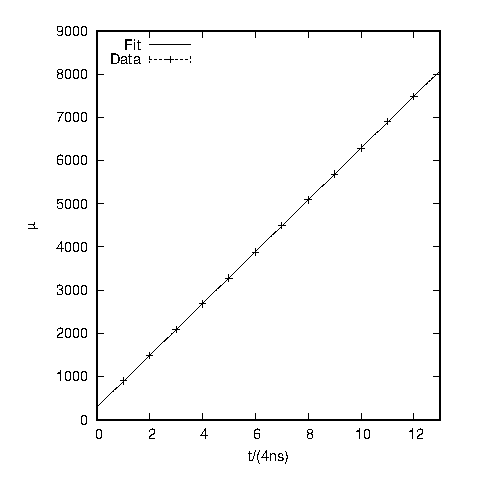
\includegraphics[width=1\linewidth]{evaluation_kilian/prompt/prompt_means.eps}
  \caption{Bin numbers $\mu_i$ against the time with fitted straight line.}
  \label{fig:prompt_fit}
\end{subfigure}%
\caption{Data and fits from the prompt curve.}
\end{figure}

To find the time per bin we plot the means $\mu_i$ in dependence of the peaknumber. Fitting (here $t$ is the time in \si{\nano\second}) 
\begin{align*}
  \mu(t)=a\cdot t+b
\end{align*}
we find that
\begin{align*}
  a&=150.0 \pm 0.1\\
  b&=287 \pm 5.
\end{align*} 
The data and the function can be found in figure \ref{fig:prompt_fit}. We conclude that \SI{1}{\nano\second} equals $150.0 \pm 0.1$ bins.

\subsection{Time Constant of Heating System}
To find the time constant of the heating system the heating was set to the lowest level and for 20 minutes every \SI{30}{\second} the temperature was measured ($\Delta T\ind{thermometer} = \SI{0.1}{\kelvin}$). The result is given in figure \ref{fig:heatcurve}. Then an exponential fit
\begin{align*}
 T(t)=B - A \cdot e^{-t/\tau\ind{heat}} 
\end{align*}
was executed on that data which resulted in 
\begin{align*}
A &= \SI[separate-uncertainty=true]{29.2(2)}{\celsius}\\
B &= \SI[separate-uncertainty=true]{55.3(1)}{\celsius}\\
\tau\ind{heat} &= \SI[separate-uncertainty=true]{245(4)}{\second}.
\end{align*}
To make sure that the temperature has stabilised within $\Delta T\ind{stabilisation} = \SI{1}{\celsius}$ we decided to wait 10 minutes before starting a measurement at a new temperature (for the indium measurement we changed the temperature by about $\SI{10}{\celsius}$). The expected deviation of the temperature is then 
\begin{align*}
\Delta T =e^{-600/245}\SI{10}{\celsius}  \approx \SI{0.86}{\celsius} < \SI{1}{\celsius}. 
\end{align*}
To make sure that the value is inside the error range we choose the error more generously, i.e.\ $\Delta T = \SI{1}{\celsius}$.

\begin{figure}[h]
\centering
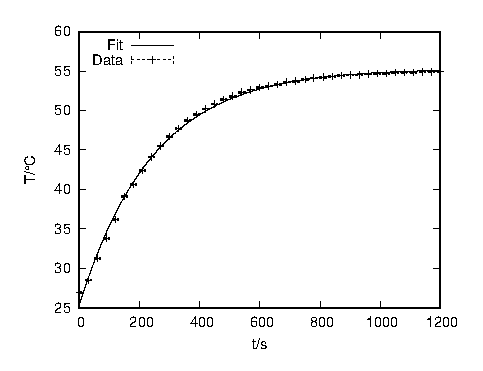
\includegraphics[width=0.6\linewidth]{auswertung/heatcurve.eps}
\caption{Heating curve and fit for evaluation of the time constant.}
\label{fig:heatcurve}
\end{figure}

\newpage

\subsection{Vacancy Formation in Indium}

The measured spectra can be found in figure \ref{fig:lifetime_spectra} in the appendix. Performing an error weighted fit with gnuplot (with the error coming from the Poisson distribution and leaving the empty bins) we fit the function $N(t)$ according to equation (\ref{eq:fit_rate}) to them. The result is given in table \ref{tab:fit_rate} in the appendix. Note that the relation $\tau_0 < \tau_\mathrm{t}$ allows us to choose the right coefficients from the fit. \\

As one can see in figure \ref{fig:indium_times} the times $\tau_0$ and $\tau_\mathrm{t}$ are uncorrelated from the temperature. We can not explain this. 

\begin{figure}[h]
\centering
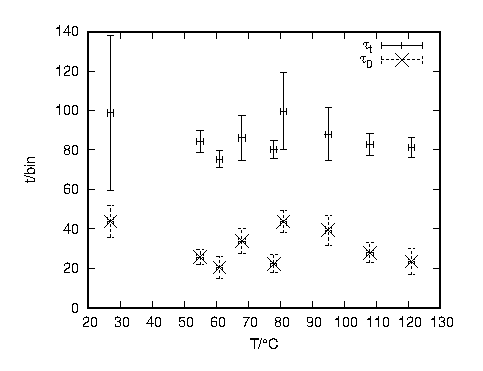
\includegraphics[width=0.6\linewidth]{auswertung/times.eps}
\caption{Lifetimes $\tau_0$ and $\tau_\mathrm{t}$ over $T$.}
\label{fig:indium_times}
\end{figure}


From the obtained values $\sigma \rho$ in units of 1/bin can be calculated according to equation (\ref{eq:transition_rate}) (errors are obtained using gaussian error propagation). The logarithm is plotted over $1/T[\si{\kelvin}]$ (see figure \ref{fig:indium_res}). We perform a linear fit 
\begin{align*}
  \log(\sigma\rho\cdot \mathrm{bin})=a \cdot \frac{1}{T}+b.
\end{align*} 
As one can see in figure \ref{fig:indium_res} the data points do not seem to lie on a line. Apart from that the resulting parameters are
\begin{align*}
  a&=\SI[separate-uncertainty=true]{-46(257)}{\kelvin}\\
  b&=(-1.6 \pm 0.7).
\end{align*}


\begin{figure}[h]
\centering
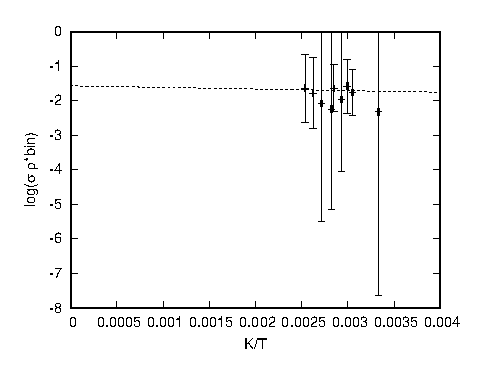
\includegraphics[width=0.6\linewidth]{auswertung/fit.eps}
\caption{Logarithmic plot of $\sigma \rho$ over $1/T$.}
\label{fig:indium_res}
\end{figure}

Using equation (\ref{eq:enthalpy}) and our result from the prompt curve we can infer that 
\begin{align*}
  \sigma e^{S_t/k_\mathrm{B}} = e^b = (0.21 \pm 0.15)/\mathrm{bin} = (32 \pm 23) /\si{\nano\second}.
\end{align*}
In \cite{weiler} the value $\sigma e^{S_t/k} = 10^8/\si{\nano\second}$ is given. Our result differs by about 7 orders of magnitude from that. We guess this is because the values of $\tau_0$ and $\tau_\mathrm{t}$ do not show a sensible dependence of the temperature. Since the fits to the time spectra look suitable we believe that the error is caused by the setup of the experiment. However, we will ignore this and continue with the evaluation of the experiment. \\

By multiplying $a$ with $k_\mathrm{B} = 1.38 \cdot 10^{-23}\,\si{\joule/\kelvin}$ \cite{pdg} we can find the vacancy formation enthalpy
\begin{align*}
  H_t =(4 \pm 22) \cdot 10^{-3}\,\si{eV}.
\end{align*}
In \cite{weiler} the vacancy formation enthalpy is given by $\SI[separate-uncertainty=true]{0.54(3)}{\electronvolt}$. This means our value differs by two orders of magnitude. But as said before we don't expect our value to be sensible because also the value for $\sigma e^{S_t/k}$ was not sensible either. 
